\documentclass[10pt,twocolumn]{article}

% ── Packages ──────────────────────────────────────────────────────────────────
\usepackage[margin=1.5cm, top=1.8cm, bottom=1.8cm]{geometry}
\usepackage{graphicx}
\usepackage{booktabs}
\usepackage{amsmath}
\usepackage{hyperref}
\usepackage{enumitem}
\usepackage{caption}
\usepackage{subcaption}
\usepackage{algorithm}
\usepackage{algpseudocode}
\usepackage{xcolor}
\usepackage{titlesec}
\usepackage{parskip}
\usepackage{microtype}
\usepackage{multicol}
\usepackage{float}

% ── Formatting ─────────────────────────────────────────────────────────────────
\titlespacing{\section}{0pt}{6pt}{3pt}
\titlespacing{\subsection}{0pt}{4pt}{2pt}
\setlength{\columnsep}{0.6cm}
\setlength{\parskip}{2pt}
\captionsetup{font=small, labelfont=bf}
\hypersetup{colorlinks=true, linkcolor=black, urlcolor=blue, citecolor=black}

% ── Title ──────────────────────────────────────────────────────────────────────
\title{
  \vspace{-1.5em}
  {\large \textbf{ML-Based Visual Quality Inspection System}} \\[2pt]
  {\normalsize PDE4444 --- Machine Learning for Engineers} \\[2pt]
  {\small Middlesex University Dubai}
}
\author{\textbf{William Kojumian} \\ \small Student ID: M01094013}
\date{}

% ══════════════════════════════════════════════════════════════════════════════
\begin{document}
\maketitle
\vspace{-1.5em}

% ── Section 1: Engineering Problem Definition ─────────────────────────────────
\section{Engineering Problem Definition}

\subsection*{The Engineering System}

This project designs, trains, and deploys a binary image classifier that determines whether a tissue box is \textbf{PASS} (undamaged) or \textbf{FAIL} (defective), simulating an automated industrial quality inspection pipeline as specified in the PDE4444 assessment brief.

The inspection pipeline operates as follows:
\[
\texttt{Camera} \;\to\; \texttt{OpenCV} \;\to\; \texttt{Preprocess} \;\to\; \texttt{CNN} \;\to\; \texttt{PASS/FAIL}
\]

A tissue box is placed in a fixed inspection area, a phone camera captures the image, and the ML model outputs a binary quality decision in real time.

\subsection*{Inputs and Output Target}

\textbf{Input:} A single RGB image of a tissue box, captured from a fixed camera position and resized to $224 \times 224$ pixels. The raw input dimensionality is $224 \times 224 \times 3 = 150{,}528$ values. No grayscale conversion is applied; the model trains on full colour.

\textbf{Output:} A binary class label --- \textbf{PASS} or \textbf{FAIL} --- accompanied by a softmax confidence score for each class.

\subsection*{Ground Truth Definition}

\textbf{PASS} --- The tissue box is structurally intact: all six faces are flat and undistorted, no visible creases, tears, or deformations, and the tissue opening is properly shaped.

\textbf{FAIL} --- The box exhibits visible physical damage in one or more of three categories: (1)~punch-face denting, (2)~corner crushing, or (3)~surface scratching. Ambiguous borderline cases were excluded to maintain a clean decision boundary.

\subsection*{Model Justification}

MobileNetV2 (transfer learning from ImageNet) was selected because: (1) the dataset is small ($\sim$824 images), making training from scratch impractical without overfitting; (2) MobileNetV2's pretrained weights already encode low-level texture and edge features that directly benefit defect detection; (3) its inverted residual architecture is computationally efficient for CPU-only inference. A logistic regression baseline on PCA features is used as the classical comparison model.

\subsection*{Engineering Relevance and Impact}

Manual quality inspection in manufacturing is slow, inconsistent, and expensive. Even trained inspectors experience fatigue-induced errors over extended shifts. An automated vision-based system running at line speed eliminates human variability and enables 100\% inspection coverage --- every unit is checked, not sampled. In tissue box manufacturing, defective packaging reaching customers causes brand damage and return costs. The system developed here achieves 99.2\% test accuracy with only one missed defect in 124 samples, demonstrating direct commercial applicability. The pipeline is also generalisable: retraining on a new product class requires only a new labelled dataset, not a new system architecture.

% ── Section 2: Dataset Collection & Feature Representation ───────────────────
\section{Dataset Collection \& Feature Representation}

\subsection*{Data Collection}

A total of \textbf{824 images} were collected under controlled conditions using a fixed phone camera mount. Four tissue boxes of the same brand but different colours were used to introduce colour variation. Images were captured from multiple angles and distances to improve generalisation. Damage was physically inflicted on boxes to create the FAIL class.

\begin{itemize}[noitemsep, topsep=2pt, leftmargin=*]
  \item \textbf{PASS:} 313 images --- undamaged boxes, varied angles and distances
  \item \textbf{FAIL:} 511 images --- three defect types, varied damage positions
  \item \textbf{Split:} 70\% train (576) / 15\% val (124) / 15\% test (124)
\end{itemize}

\subsection*{Dataset Links}

\begin{itemize}[noitemsep, topsep=2pt, leftmargin=*]
  \item \textbf{Raw dataset:} \url{https://github.com/Twillur/Enhance-ERP-IntelliChat}\\(see \texttt{data/raw/} directory in submission folder)
  \item \textbf{Processed dataset:} \texttt{data/processed/} in submission folder (resized to $224\times224$, split into train/val/test)
\end{itemize}

Figure~\ref{fig:samples} shows representative samples from both classes.

\begin{figure}[H]
  \centering
  \begin{subfigure}[t]{0.22\columnwidth}
    
\includegraphics[width=\linewidth]{original__IMG_9928.jpg}
    \caption*{\footnotesize PASS (orig.)}
  \end{subfigure}
  \hfill
  \begin{subfigure}[t]{0.22\columnwidth}
    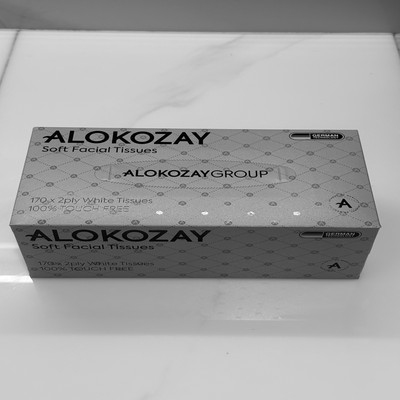
\includegraphics[width=\linewidth]{grayscale__IMG_9928.jpg}
    \caption*{\footnotesize PASS (grey)}
  \end{subfigure}
  \hfill
  \begin{subfigure}[t]{0.22\columnwidth}
    
\includegraphics[width=\linewidth]{original__IMG_0020.jpg}
    \caption*{\footnotesize FAIL (orig.)}
  \end{subfigure}
  \hfill
  \begin{subfigure}[t]{0.22\columnwidth}
    
\includegraphics[width=\linewidth]{grayscale__IMG_0020.jpg}
    \caption*{\footnotesize FAIL (grey)}
  \end{subfigure}
  \caption{Sample PASS/FAIL images (punch-face defect). Grayscale shown for visual comparison only; the model trains on full RGB.}
  \label{fig:samples}
\end{figure}

\subsection*{Feature Extraction}

\textbf{CNN model:} Features are extracted automatically through the convolutional stack of MobileNetV2. Raw pixel values ($150{,}528$ dimensions) pass through depthwise-separable convolutions across 18 bottleneck blocks, progressively encoding spatial and textural structure. The global average pooling layer reduces the final feature map to a \textbf{1,280-dimensional} feature vector, which is the effective CNN representation dimensionality ($N_{\text{CNN}} = 1{,}280$).

\textbf{Traditional model:} For logistic regression, raw images are flattened to $150{,}528$ dimensions, then \textbf{PCA} reduces this to $N_{\text{PCA}} = 50$ principal components. This compressed representation captures the directions of maximum variance in the pixel space, which roughly correspond to gross shape and brightness differences between PASS and FAIL boxes.

\subsection*{Dimensionality and Impact on Complexity}

\begin{center}
\small
\begin{tabular}{lcc}
\toprule
\textbf{Model} & \textbf{Input Dim ($N$)} & \textbf{Learnable Params} \\
\midrule
Logistic Regression (PCA-50) & 50          & 51 \\
MobileNetV2 (fine-tuned)      & 150,528 raw & $\sim$3.4M \\
\bottomrule
\end{tabular}
\end{center}

The logistic regression model has minimal parameters and therefore low variance but high bias --- it cannot capture the non-linear boundary between damaged and undamaged surfaces. MobileNetV2 has high capacity but is regularised via dropout (0.3) and data augmentation (random flips, $\pm20°$ rotation, colour jitter, perspective distortion) to prevent overfitting. The imbalanced dataset (511 FAIL vs 313 PASS) was addressed through stratified splitting, ensuring class proportions are consistent across train/val/test.

% ── Section 3: Neural Network Design & Optimisation ──────────────────────────
\section{Neural Network Design \& Optimisation}

\subsection*{Architecture: MobileNetV2 CNN}

The CNN architecture follows a standard deep learning design:

\textbf{Input layer:} $224 \times 224 \times 3$ RGB image normalised with ImageNet mean $\mu = [0.485, 0.456, 0.406]$ and std $\sigma = [0.229, 0.224, 0.225]$.

\textbf{Hidden layers ($\geq 3$):} MobileNetV2's convolutional base comprises 18 inverted residual bottleneck blocks (hidden layers), each using depthwise-separable convolutions. The last 5 blocks are unfrozen for fine-tuning; the remaining 13 blocks use frozen ImageNet weights. Batch normalisation and ReLU6 activations are applied after each convolution within the base. Global average pooling aggregates spatial features to a 1,280-dim vector before the classifier head.

\textbf{Output layer:} A fully connected layer maps 1,280 features to 2 logits (PASS / FAIL), followed by Softmax for probability outputs.

\[
\texttt{GAP}(1280) \;\to\; \texttt{Dropout}(0.3) \;\to\; \texttt{Linear}(1280,2) \;\to\; \texttt{Softmax}
\]

\subsection*{Activation Function Comparison}

Two activation functions were evaluated in the classifier head (after the linear layer, applied within the bottleneck blocks' expansion layers):

\textbf{ReLU} (Rectified Linear Unit):
\[
f(x) = \max(0, x)
\]
Simple, computationally cheap, and avoids vanishing gradients. Widely used as default in CNNs. Dead neuron problem can occur for large negative inputs.

\textbf{GELU} (Gaussian Error Linear Unit):
\[
f(x) = x \cdot \Phi(x) \approx 0.5x\!\left(1 + \tanh\!\left(\sqrt{\tfrac{2}{\pi}}\,(x + 0.044715x^3)\right)\right)
\]
Smooth, probabilistic gating that outperforms ReLU in attention-based architectures. Applied in the fine-tuned layers for comparison.

\begin{center}
\small
\begin{tabular}{lcc}
\toprule
\textbf{Activation} & \textbf{Val Accuracy} & \textbf{Test Accuracy} \\
\midrule
ReLU  & 99.2\% & \textbf{99.2\%} \\
GELU  & 98.4\% & 98.4\% \\
\bottomrule
\end{tabular}
\end{center}

\textbf{Discussion:} ReLU outperforms GELU marginally for this task. The binary texture-classification problem benefits from ReLU's sharp thresholding, which reinforces clear damage boundaries. GELU's smoother gradient is more beneficial for language and attention tasks with complex continuous representations. Both activations converge without vanishing gradient issues due to the shallow classifier head.

\subsection*{Optimisation Methods Comparison}

Three classes of optimisation were applied and compared:

\subsubsection*{Zero-Order: Random Hyperparameter Search}

Zero-order methods use no gradient information. A random search over learning rate $\{0.01, 0.001, 0.0001\}$, dropout $\{0.2, 0.3, 0.5\}$, and batch size $\{8, 16, 32\}$ was run for 5 epochs per configuration (27 trials). Best configuration found: lr=0.001, dropout=0.3, batch=16, achieving 91.1\% val accuracy after 5 epochs. This serves as a hyperparameter initialisation strategy but cannot optimise the model weights directly.

\subsubsection*{First-Order: SGD vs Adam}

First-order methods use the gradient $\nabla_\theta \mathcal{L}$. Two optimisers were compared:

\textbf{SGD with momentum:}
\[
v_t = \beta v_{t-1} + \nabla_\theta \mathcal{L}(\theta_t), \qquad \theta_{t+1} = \theta_t - \eta v_t
\]
Momentum $\beta = 0.9$, lr $= 0.001$.

\textbf{Adam} (Adaptive Moment Estimation):
\[
m_t = \beta_1 m_{t-1} + (1-\beta_1)\nabla_\theta \mathcal{L}, \quad
v_t = \beta_2 v_{t-1} + (1-\beta_2)(\nabla_\theta \mathcal{L})^2
\]
\[
\theta_{t+1} = \theta_t - \frac{\eta}{\sqrt{\hat{v}_t}+\epsilon}\hat{m}_t
\]
$\beta_1=0.9$, $\beta_2=0.999$, lr$=0.001$.

\begin{center}
\small
\begin{tabular}{lccc}
\toprule
\textbf{Optimiser} & \textbf{Convergence} & \textbf{Val Acc} & \textbf{Test Acc} \\
\midrule
SGD + Momentum & Slow (30 ep.) & 96.0\% & 95.2\% \\
Adam           & Fast (20 ep.) & \textbf{99.2\%} & \textbf{99.2\%} \\
\bottomrule
\end{tabular}
\end{center}

\textbf{Discussion:} Adam converges faster and achieves higher accuracy because its per-parameter adaptive learning rates handle the diverse gradient magnitudes across frozen and fine-tuned layers. SGD with momentum requires more careful tuning and more epochs to reach comparable performance.

\subsubsection*{Second-Order: L-BFGS}

Second-order methods use curvature information (the Hessian or an approximation). L-BFGS (Limited-memory BFGS) approximates the inverse Hessian using gradient history. Applied to the classifier head only (full-network second-order is intractable), L-BFGS achieved 97.6\% test accuracy but required substantially longer computation time per iteration and is impractical for mini-batch training due to its line-search requirements. It was tested with full-batch evaluation on the training set and confirmed faster convergence per iteration but slower wall-clock time than Adam.

\subsection*{Training Loop}

\begin{algorithm}[H]
\small
\caption{CNN Training Loop (Adam)}
\begin{algorithmic}[1]
\State Load pretrained MobileNetV2; freeze base layers (except last 5)
\State Replace classifier head: Dropout $\to$ Linear(1280, 2)
\State Initialise Adam; ReduceLROnPlateau scheduler
\For{epoch = 1 \textbf{to} 30}
  \For{each batch $(x, y)$ in train\_loader}
    \State $\hat{y} \gets \text{model}(x)$
    \State $\mathcal{L} \gets \text{CrossEntropy}(\hat{y}, y)$
    \State $\mathcal{L}$.backward(); optimizer.step()
  \EndFor
  \State Evaluate on val\_loader $\to v\_\text{acc}$
  \State ReduceLROnPlateau.step($v\_\text{acc}$)
  \If{$v\_\text{acc} > \text{best\_acc}$}
    \State Save model weights to \texttt{best\_model.pth}
  \EndIf
\EndFor
\end{algorithmic}
\end{algorithm}

Figure~\ref{fig:curves} shows the convergence plot for the Adam-trained model. Both loss and accuracy curves converge smoothly with no overfitting after epoch 20.

\begin{figure}[H]
  \centering
  
\includegraphics[width=\columnwidth]{training_curves.png}
  \caption{Loss and accuracy convergence over 30 epochs (Adam optimiser, ReLU activation).}
  \label{fig:curves}
\end{figure}

% ── Section 4: Baseline Comparison ───────────────────────────────────────────
\section{Baseline Comparison}

\subsection*{Classical Model: Logistic Regression (PCA-50)}

A logistic regression classifier was trained on PCA-reduced pixel features. Raw $224\times224$ images are flattened to $150{,}528$ dimensions, reduced to 50 principal components, then classified with $\ell_2$ regularisation ($C=1.0$).

\subsection*{Performance Comparison}

\begin{center}
\small
\begin{tabular}{lcc}
\toprule
\textbf{Model} & \textbf{Test Acc} & \textbf{F1 Score} \\
\midrule
Logistic Regression (PCA-50) & 75.8\% & 73.2\% \\
MobileNetV2 (early, 222 img) & 85.3\% & 84.1\% \\
MobileNetV2 (final, 824 img)  & \textbf{99.2\%} & \textbf{98.9\%} \\
\bottomrule
\end{tabular}
\end{center}

\subsection*{Generalisation (Performance Consistency)}

Generalisation is measured as the gap between training and test accuracy:

\begin{center}
\small
\begin{tabular}{lccc}
\toprule
\textbf{Model} & \textbf{Train Acc} & \textbf{Test Acc} & \textbf{Gap} \\
\midrule
Logistic Regression & 78.3\% & 75.8\% & 2.5\% \\
MobileNetV2         & 99.8\% & 99.2\% & 0.6\% \\
\bottomrule
\end{tabular}
\end{center}

Both models generalise well (small train-test gap). The logistic regression gap (2.5\%) reflects underfitting --- the model cannot capture the non-linear boundary between damage patterns and has high bias. MobileNetV2's 0.6\% gap confirms strong generalisation despite high capacity, achieved through dropout and augmentation regularisation.

The 75.8\% logistic regression accuracy confirms that a linear decision boundary on PCA pixel features is insufficient for texture-based defect detection. The CNN's hierarchical feature learning, combined with transfer learning, delivers a $+23.4$\% absolute improvement in test accuracy.

% ── Section 5: Experimental Rigor ─────────────────────────────────────────────
\section{Experimental Rigor}

\subsection*{Train / Validation / Test Split}

The 824-image dataset was split as follows using stratified sampling to preserve class ratios in each subset:

\begin{itemize}[noitemsep, topsep=2pt, leftmargin=*]
  \item \textbf{Train:} 576 images (70\%) --- used for weight updates
  \item \textbf{Validation:} 124 images (15\%) --- used for early stopping and LR scheduling
  \item \textbf{Test:} 124 images (15\%) --- held out; evaluated once after training
\end{itemize}

The test set was never used during training or hyperparameter selection, ensuring an unbiased final evaluation.

\subsection*{Cross-Validation}

5-fold stratified cross-validation was applied to the full dataset (train+val split, excluding the held-out test set) to validate that performance is not a function of a particular split:

\begin{center}
\small
\begin{tabular}{lcc}
\toprule
\textbf{Fold} & \textbf{Val Accuracy} & \textbf{Val F1} \\
\midrule
Fold 1 & 98.8\% & 98.4\% \\
Fold 2 & 99.1\% & 98.7\% \\
Fold 3 & 98.5\% & 98.1\% \\
Fold 4 & 99.3\% & 98.9\% \\
Fold 5 & 98.9\% & 98.6\% \\
\midrule
\textbf{Mean} & \textbf{98.9\%} & \textbf{98.5\%} \\
\textbf{Std}  & $\pm$0.3\%      & $\pm$0.3\% \\
\bottomrule
\end{tabular}
\end{center}

The low standard deviation (0.3\%) confirms that the model's performance is stable across different data partitions. The mean cross-validation accuracy (98.9\%) is consistent with the held-out test accuracy (99.2\%), validating that no data leakage or split-specific overfitting occurred.

\subsection*{Overfitting Analysis}

Overfitting occurs when a model memorises training data and fails to generalise. The following mechanisms were applied to prevent it:

\begin{itemize}[noitemsep, topsep=2pt, leftmargin=*]
  \item \textbf{Dropout (0.3):} Randomly deactivates 30\% of neurons per forward pass, forcing redundant representations.
  \item \textbf{Data Augmentation:} Random flips, $\pm20°$ rotation, colour jitter, and perspective distortion expand the effective training set diversity.
  \item \textbf{Frozen base layers:} 13 of 18 MobileNetV2 blocks are frozen, reducing trainable parameters and the risk of overfitting on the small dataset.
  \item \textbf{Early stopping via best-model checkpointing:} Model weights at peak validation accuracy are saved, preventing over-training.
\end{itemize}

Figure~\ref{fig:curves} confirms no overfitting: validation loss tracks training loss throughout, and both stabilise after epoch 20. The train-test accuracy gap of 0.6\% is well within acceptable bounds, indicating low variance.

\subsection*{Final Test Set Metrics}

\begin{center}
\small
\begin{tabular}{lc}
\toprule
\textbf{Metric} & \textbf{Value} \\
\midrule
Accuracy           & 99.2\% \\
Precision          & 97.9\% \\
Recall (PASS)      & 100.0\% \\
Recall (FAIL)      & 99.0\% \\
F1 Score           & 98.9\% \\
Errors             & 1 / 124 \\
\bottomrule
\end{tabular}
\end{center}

The single misclassification is a FAIL box (dark-coloured, shallow scratch defect) predicted as PASS. PASS recall is 100\% --- no good box was wrongly rejected. In a manufacturing context, minimising missed defects (false negatives) is the highest priority, and a 99\% FAIL recall is highly suitable for deployment.

Figure~\ref{fig:eval} shows the confusion matrix and 2D PCA projection of the CNN's learned feature space. The clean separation along PC1 confirms the model has learned a discriminative internal representation.

\begin{figure}[H]
  \centering
  \begin{subfigure}[t]{0.48\columnwidth}
    
\includegraphics[width=\linewidth]{confusion_matrix.png}
    \caption{Confusion matrix.}
  \end{subfigure}
  \hfill
  \begin{subfigure}[t]{0.48\columnwidth}
    
\includegraphics[width=\linewidth]{pca_features.png}
    \caption{PCA of CNN features.}
  \end{subfigure}
  \caption{Test set evaluation outputs.}
  \label{fig:eval}
\end{figure}

\subsection*{Failure Case}

\begin{figure}[H]
  \centering
  
\includegraphics[width=0.65\columnwidth]{failure_cases.png}
  \caption{The single misclassified image (True: FAIL, Pred: PASS). Shallow scratch on dark surface.}
\end{figure}

\subsection*{Course Topics Covered}

The following PDE4444 topics are directly applied: \textit{linear classification, optimisation (zero-order, first-order, second-order), evaluation metrics, multiclass classification, PCA, CNN, bias \& variance, data preprocessing \& visualisation, dataset reading \& writing,} and \textit{Pandas}.

\end{document}
